\documentclass{article}
\usepackage{amsmath}
\usepackage{graphicx}
\usepackage[utf8]{inputenc}
\usepackage[T1, T2A]{fontenc}
\usepackage[english,russian]{babel}

\title{Задачи к теорминимуму}
\author{Anikin Evgeny, 121}

\begin{document}
\maketitle
\section{Задача 1}
	\subsection{Ответ}
	\begin{equation}
		\frac{\sqrt{U_0} - \sqrt{|E|}}{\alpha} = \mathrm{const} 
	\end{equation}
	\subsection{Решение}
	Нужно найти адиабатический инвариант частицы в потенциале
	\begin{equation}
		U(x) = U_0 ( e^{-2\alpha x} - 2 e^{-\alpha x})
	\end{equation}
	Соответствующий лагранжиан выглядит так:
	\begin{equation}
		L = \frac{m\dot{x}^2}{2} - U(x)
	\end{equation}
	Удобно сделать подстановку
	\begin{equation}
		q = e^{-\alpha x} ,
	\end{equation}
	\begin{equation}
		\dot{q} = -\alpha \dot{x} e^{-\alpha x} = - \alpha q \dot{x},
	\end{equation}
	так что новый лагранжиан получается таким:
	\begin{equation}
		L = \frac{m\dot{q}^2}{2\alpha^2 q^2} - U_0( q^2 - 2 q ). 
	\end{equation}
	Гамильтониан ---
	\begin{equation}
		\label{Ham}
		H = \frac{\alpha^2 p^2 q^2}{2m} + U_0(q^2 - 2q)
	\end{equation}
	Движение частицы финитно, если выполняется неравенство
	$-U_0 < E < 0$. 

	Получим выражение для импульса из формулы \ref{Ham}:
	\begin{equation}
		p = \frac{\sqrt{2mU_0}}
		{\alpha} \frac{\sqrt{-q^2 + 2q - |E|/U_0}}{q}
	\end{equation}
	Частица движется между точками $q_1$, $q_2$, которые определяются из уравнения 
	\begin{equation}
		q^2 - 2q + \frac{|E|}{U_0} = 0
	\end{equation}
	\begin{equation}
		q_{1,2} = 1 \pm \sqrt{1 - \frac{|E|}{U_0}}
	\end{equation}
	Оба корня $q_1, q_2$ больше нуля.
	
	Адиабатический инвариант --- 
	\begin{equation}
		\label{inv}
		A = \int p\,dq = \frac{2\sqrt{2mU_0}}{\alpha} 
					\int\frac{\sqrt{-q^2 + 2q - |E|/U_0}}{q}\,dq
	\end{equation}

	Этот интеграл можно взять как контурный:
	\begin{figure}[h]
		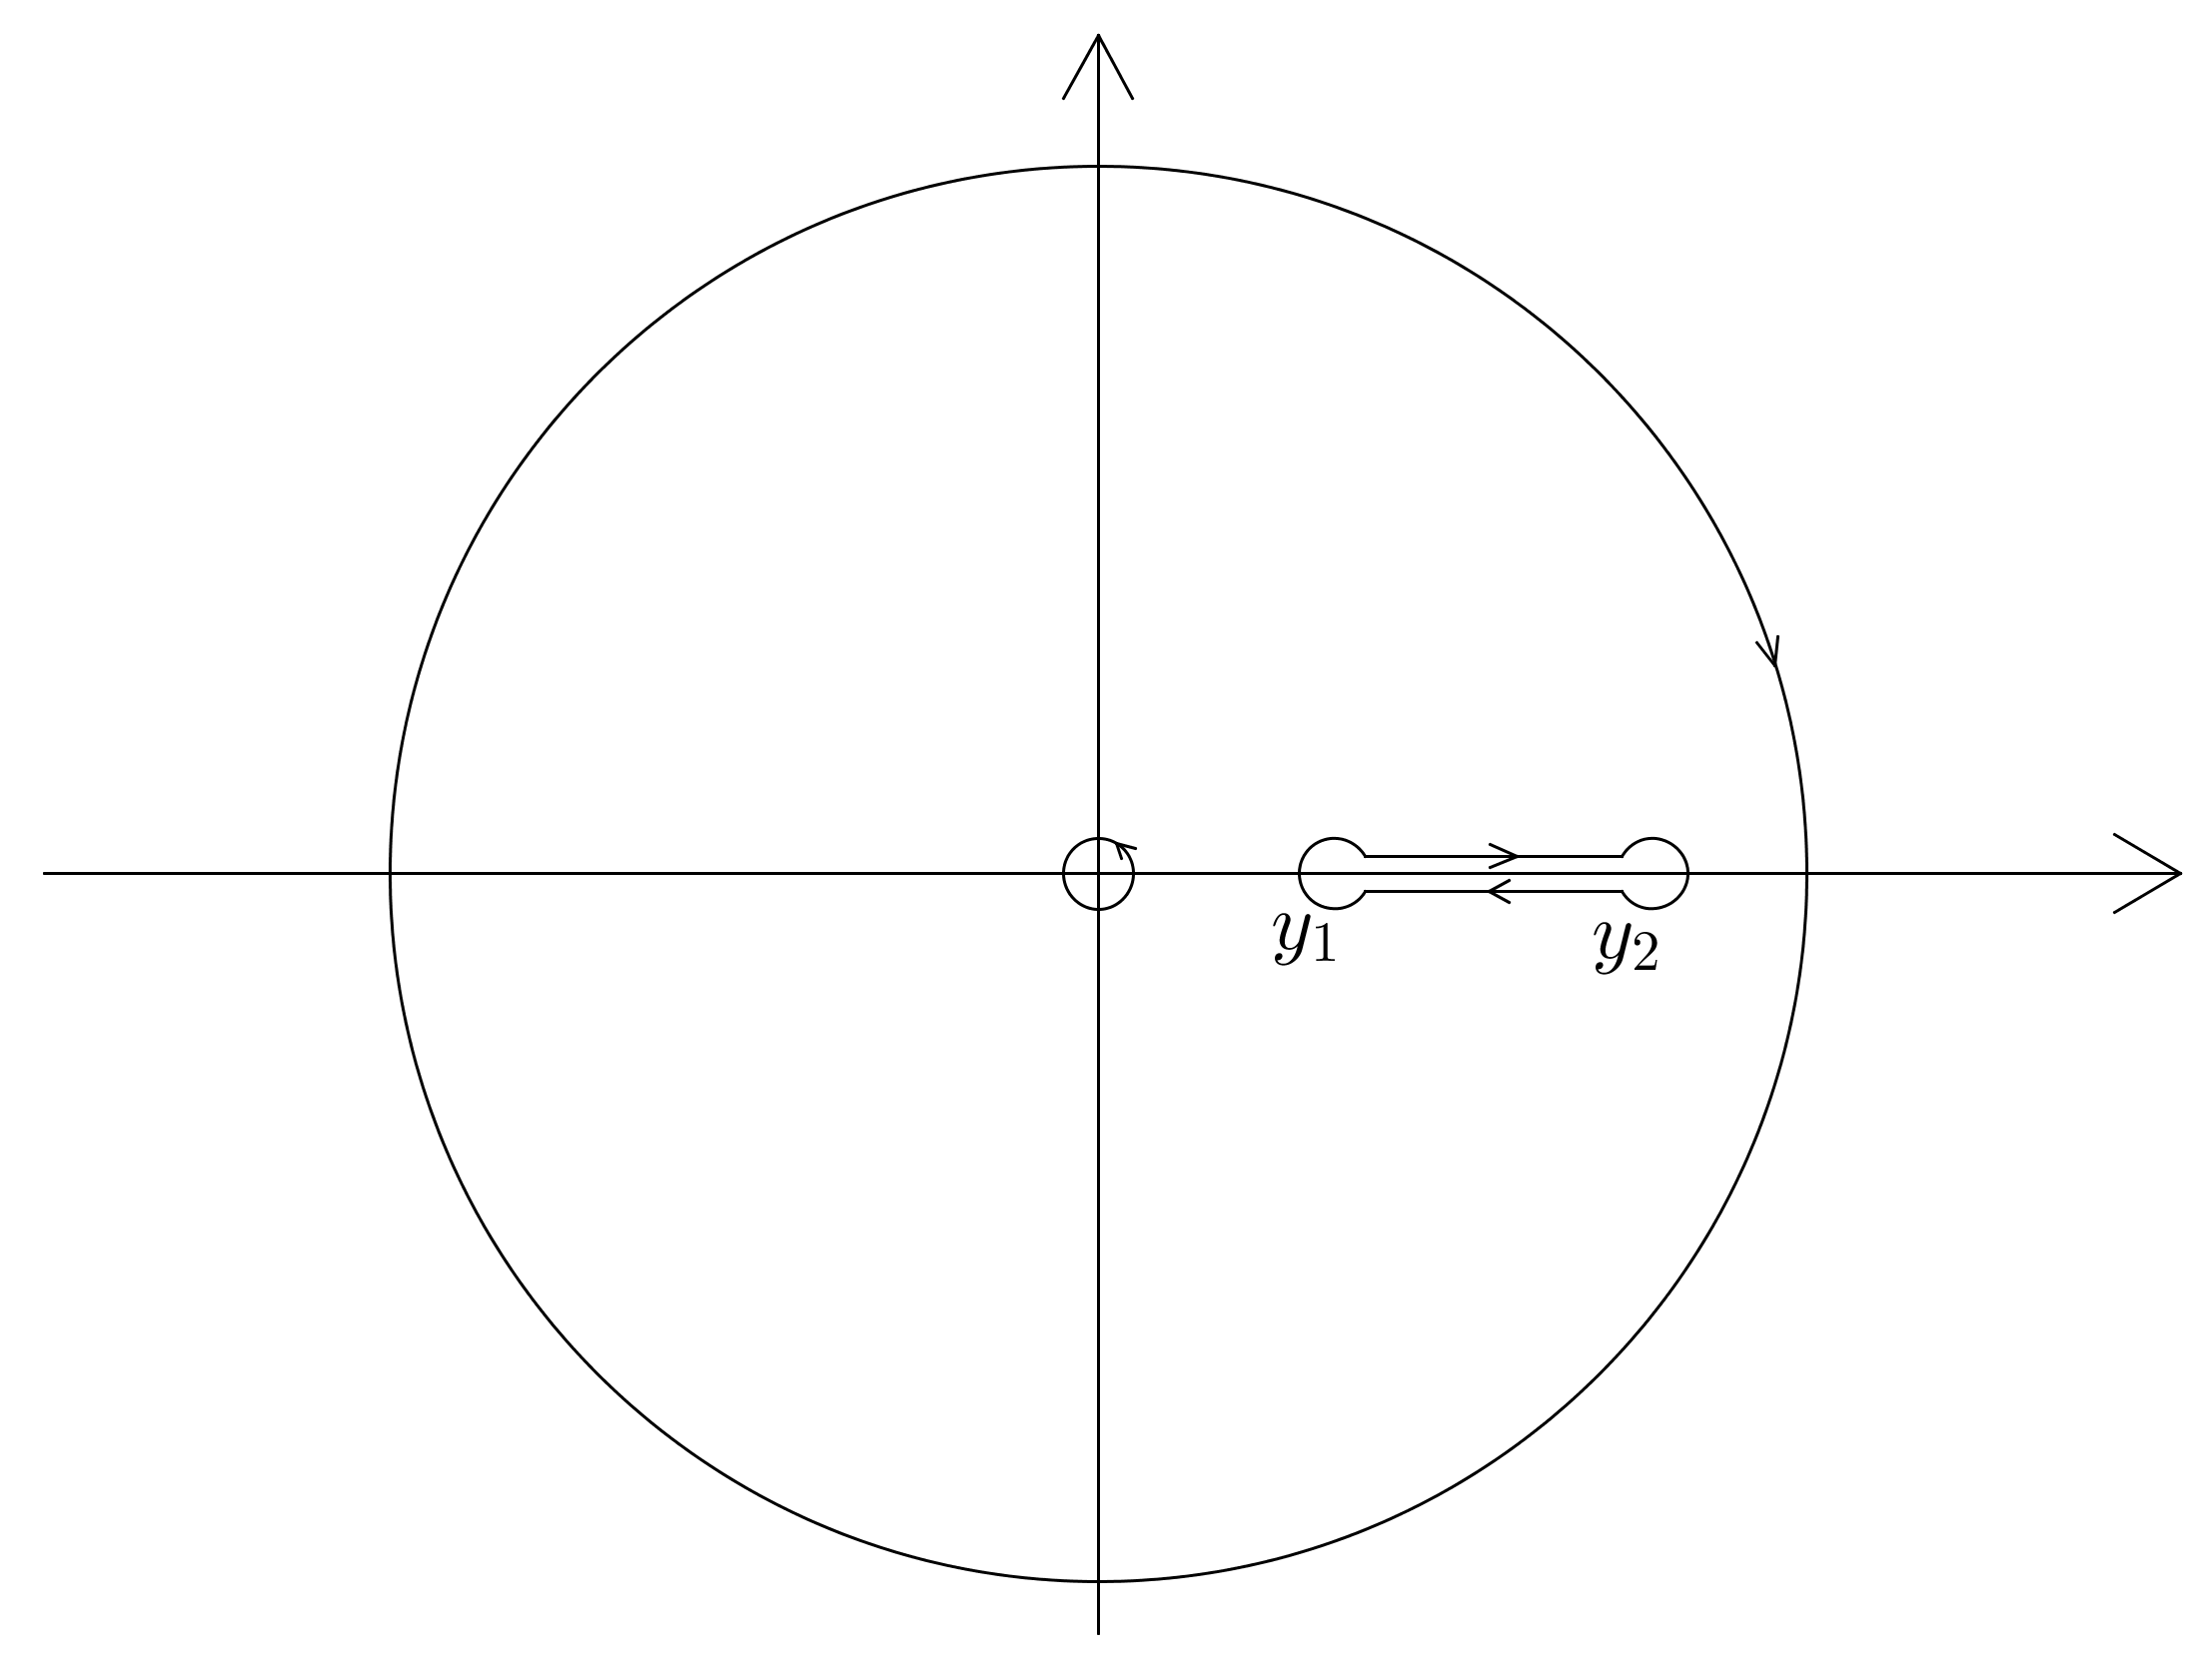
\includegraphics[width=\linewidth]{contour.png}
	\end{figure}

	Для вычисления интеграла нужны вычеты функции
	\begin{equation}
		F(q) = \frac{\sqrt{-q^2 + 2q - |E|/U_0}}{q}
	\end{equation}
	в точках $0$, $\infty$.
	При $q < q_1$ ветвь  
	функции $F(q) = i\sqrt{q^2 - 2q + |E|/U_0}$,
	а при $q > q_2$ --- $F(q) = -i\sqrt{q^2 - 2q + |E|/U_0}$.
	Вычет в точке $q = 0$ даётся выражением 
	\begin{equation}
		\mathrm{res}_{q = 0} F = i\sqrt{|E|/U_0}
	\end{equation}
	Для $q = \infty$ нужно немного больше работы. Необходимо
	разложить $F(q)$ в ряд Лорана. Рассмотрим большие положительные  
	$q$. Для таких $q$ имеем
	\begin{multline}
		F(q) = -i\sqrt{1 - \frac{2}{q} + \frac{|E|}{U_0q^2}} = 
		\\ 
		= -i\left(1 - \frac{1}{q} + O\left(\frac{1}{q^2}\right)\right)
		\\	
	\end{multline}
	Таким образом
	\begin{equation}
		\mathrm{res}_{q = \infty} F = i.
	\end{equation}
	Теперь продолжим равенство \ref{inv}:
	\begin{multline}
			A = \int p\,dq = \frac{1}{2}\frac{2\sqrt{2mU_0}}{\alpha} 
				\times
				2\pi i (\mathrm{res}_{q = 0}F - \mathrm{res}_{q = \infty}F)=
				\\	
				= \frac{2\pi \sqrt{2mU_0}}{\alpha}(-\sqrt{|E|/U_0}+ 1) = 
				\\
				= 2\pi \sqrt{2m}\cdot\frac{\sqrt{U_0} - \sqrt{|E|}}{\alpha} = \mathrm{const}. 
	\end{multline}
	Последнее равенство и есть ответ.
	\section{Задача 2}
	\subsection{Ответ}
	Колесо не проскальзывает, если выполняется неравенство
	\begin{equation}
		k > \frac{\epsilon}{3} 
			\frac{2gR - v^2}{\sqrt{(gR)^2 - (2\epsilon v^2)^2}}
	\end{equation}
	Предполагается, что $\omega^2 \gg gh$.
	Обозначения см. ниже.
	\subsection{Решение}
	Примем следующие обозначения: пусть $R+h$, $R-h$ --- полуоси эллиптического колеса,
	$\alpha$ --- угол поворота, $x$, $y$ --- координаты центра масс колеса, $\xi$ --- смещение
	центра масс относительно точки касания по горизонтали (см. рисунок). 
	\begin{figure}[h]
		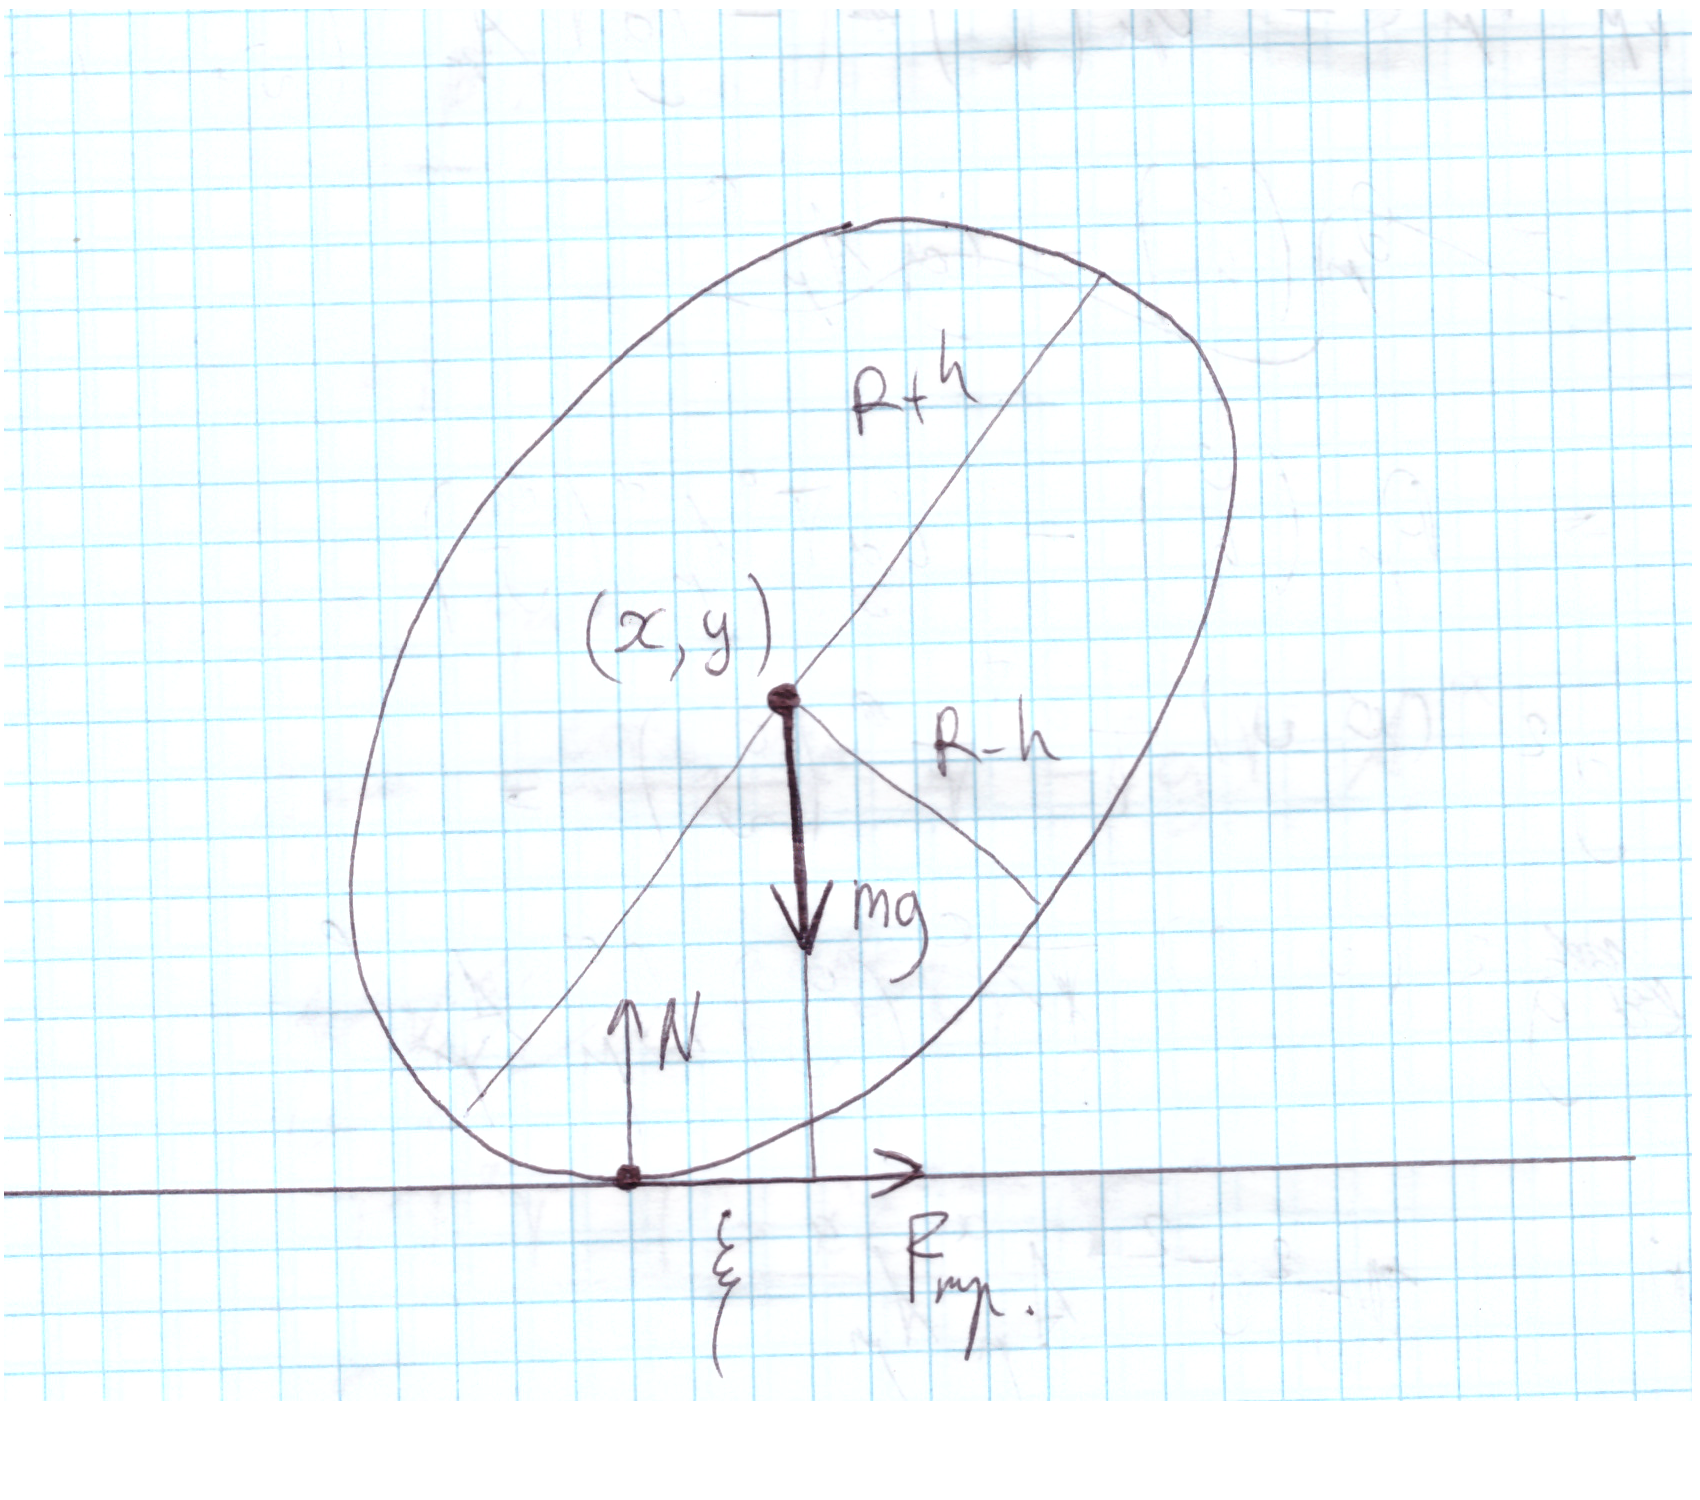
\includegraphics[width=\linewidth]{ellipsis.png}
	\end{figure}
	Будем считать, что скорость колеса достаточно велика, то есть $v^2 \gg gh$. Это значит,
	что можно будет приближённо считать скорость постоянной.

	Так как $h \ll R$, можно использовать выражения для радиуса и длины эллипса в зависимости
	от угла в первом порядке по $h/R$.
	
	\begin{equation}
		\label{rad}
		r(\alpha) = R\left(1 + \frac{h}{R} \cos{2\alpha} + O\left(\frac{h^2}{R^2}\right)\right)
	\end{equation}
	\begin{equation}
		l(\alpha) = R\left(\alpha + \frac{h}{2R} \sin{2\alpha} + 
		O\left(\frac{h^2}{R^2}\right)\right)
	\end{equation}
	\begin{equation}
		\label{xi}
		\xi(\alpha) = R\left(\frac{2h}{R} \sin{2\alpha} + O\left(\frac{h^2}{R^2}\right)\right)
	\end{equation}
	В первом порядке можно считать, что $x = l$, $y = r$. 
	Теперь напишем законы Ньютона для колеса.
	\begin{equation}
		I\dot{\omega} = N\xi - F_{\mathrm{tr}}y
	\end{equation}
	\begin{equation}
		m\ddot{x} = F_{\mathrm{tr}}
	\end{equation}
	\begin{equation}
		m\ddot{y} = -mg + N
	\end{equation}
	Исключая силы трения и реакции опоры, получим уравнение
	\begin{equation}
		I\dot{\omega} = m(\ddot{y} + g)\xi - m\ddot{x}y
	\end{equation}
	Используя очевидные равенства $\ddot{x} = x''\omega^2 + x'\dot{\omega}$, 
	$\ddot{y} = y''\omega^2 + y'\dot{\omega}$ (штрихи означают
	производную по углу $\alpha$), можно выразить угловое ускорение через
	угловую скорость и угол.
	\begin{equation}	
		\dot{\omega} = \frac{(y''\xi - x''y)\omega^2 + g\xi  }{ I/m - y'\xi + x'y }
	\end{equation}
	Пользуясь формулами \ref{rad} -- \ref{xi}, 	
	\begin{equation}
		x' = R + h\cos{2\alpha}
	\end{equation}
	\begin{equation}
		x'' = -2h\sin{2\alpha}
	\end{equation}
	\begin{equation}
		y' = -2h\sin{2\alpha}
	\end{equation}
	\begin{equation}
		y'' = -4h\cos{2\alpha}
	\end{equation}
	получим окончательное выражение для
	углового ускорения в первом порядке:
	\begin{equation}
		\dot{\omega} = \frac{2h\sin{2\alpha}(R\omega^2  + g)}{\frac{I}{m} + R^2}	
	\end{equation}
	Теперь легко выразить $\ddot{x}$ и $\ddot{y}$.
	\begin{multline}
		\ddot{x} = -2h\sin{2\alpha}\omega^2 + 
		R \frac{2h\sin{2\alpha}(R\omega^2  + g)}{\frac{I}{m} + R^2}	=
		 2h\sin{2\alpha} \frac{mgR - I\omega^2}{I + mR^2}
	\end{multline}	
	\begin{equation}
		\ddot{y} = -4h\cos{2\alpha} \omega^2
	\end{equation}	
	Условие того, что колесо не проскальзывает, можно записать так:
	\begin{equation}
		k > \left|\frac{\ddot{x}}{\ddot{y} + g}\right| = 
		\left| \frac{2h\sin{2\alpha}}{g - 4h\omega^2\cos{2\alpha}}
			\frac{mgR - I\omega^2}{I + mR^2}\right|
	\end{equation}
	или
	\begin{equation}
		\label{ineq}
		k >
		\left| \frac{2gR - v^2}{3}
		\frac{\epsilon\sin{2\alpha}}{gR - 2\epsilon v^2\cos{2\alpha}}\right|
	\end{equation}
	Если скорость считать постоянной, то нужно найти угол, при котором выражение 
	в правой части предыдущего равенства максимально.
	Дифференцируя правую часть, приходим к условию
	\begin{equation}
		\cos{2\alpha} = \frac{2\epsilon v^2}{gR}
	\end{equation}
	Подставляя в \ref{ineq}, получим
	\begin{equation}
		k > \frac{\epsilon}{3} 
			\frac{2gR - v^2}{\sqrt{(gR)^2 - (2\epsilon v^2)^2}}
	\end{equation}

	При $v^2 = 2gR$ сила трения обращается в нуль в первом порядке по $h$.
	Поэтому минимальный коэффициент трения тоже равен нулю в первом порядке.
	
	При $v^2 = \frac{gR}{2\epsilon}$ обращается в нуль сила реакции опоры. Это значит, что 
	колесо начнёт подпрыгивать.
\end{document}
